\section{Objetivo y datos del sprint}
\label{sec:introduccion}
\label{sec:datos}

El sprint evalúa si las características geométricas derivadas reducen el error de predicción de la \textbf{carga de primera falla} frente a las medidas originales. Se comparan cuatro representaciones con el mismo regresor Ridge, parámetros y particiones. También se comparan cinco algoritmos sobre geometría original, examinando sus arquitecturas, errores y capacidad de generalización. El EDA orienta las hipótesis y la evaluación fuera de muestra contrasta su utilidad, sin atribuir causalidad mecánica a las asociaciones.

Las estructuras pantográficas son mallas de fibras conectadas por pivotes deformables. Los especímenes de poliamida, fabricados mediante sinterización láser selectiva, tienen dimensiones exteriores nominales de $210\times70$~mm. Se ensayaron a tracción con carga--descarga, velocidad de desplazamiento de 15~mm/min y niveles separados cada 10~mm; se registraron fuerza--desplazamiento y eventos de rotura \cite{venditti2025}.

Cada fila representa un caso experimental. Las \textbf{familias $Y=4,5,6$} agrupan estructuras con igual cantidad de celdas en esa dirección; dentro de cada familia cambian dimensiones de fibras y pivotes. Las configuraciones se definen por $(n_Y,h_f,h_p)$, combinación de celdas, altura de fibra y altura de pivote. La coincidencia de esos factores no certifica réplica física ni igualdad de toda la geometría. Esta distinción determina la agrupación durante la validación.

Las entradas de la Tabla~\ref{tab:entradas} están disponibles antes del ensayo. El objetivo es una fuerza en N asociada a la primera rotura identificada de una fibra o pivote; no representa necesariamente el máximo global ni el colapso final. Identificadores, cargas posteriores, desplazamientos y energías quedan fuera de los predictores. El análisis se limita al dominio experimental disponible: la validación interna no demuestra transferencia a otros materiales o campañas. Como las hipótesis provienen del EDA completo, los resultados tienen carácter exploratorio.

\begin{table}[htbp]
\centering\small\setstretch{1.0}
\caption{Variables del sprint: diez entradas geométricas y una respuesta experimental.}
\label{tab:entradas}
\begin{tabularx}{\linewidth}{@{}l l X@{}}
\toprule
Variable original & Unidad & Significado y rol \\
\midrule
\texttt{n\_cells\_Y} & conteo & Entrada: celdas en Y; arquitectura de la malla. \\
\texttt{Fiber\_height} & mm & Entrada: altura $h$ de la sección de fibra. \\
\texttt{Fiber\_base} & mm & Entrada: ancho $b$ de la sección de fibra. \\
\texttt{Fiber\_total\_length} & mm & Entrada: longitud total de fibras. \\
\texttt{Fiber\_total\_volume} & mm$^3$ & Entrada: volumen de fibras, $V_f$. \\
\texttt{Pivot\_height} & mm & Entrada: altura de pivotes. \\
\texttt{Pivot\_radius} & mm & Entrada: radio de pivotes; constante. \\
\texttt{Pivot\_total\_number} & conteo & Entrada: cantidad de pivotes. \\
\texttt{Pivot\_total\_volume} & mm$^3$ & Entrada: volumen de pivotes, $V_p$. \\
\texttt{Sample\_total\_volume} & mm$^3$ & Entrada: volumen CAD; distinto de $V_f+V_p$. \\
\texttt{First\_Failure\_Load\_N} & N & Objetivo: carga de primera falla. \\
\bottomrule
\end{tabularx}
\par\smallskip\small Fuente: diccionario y tabla analítica del repositorio. Los valores geométricos son descriptores declarados; el radio se conserva en la fuente y se filtra dentro del entrenamiento.
\end{table}

\section{Análisis exploratorio y decisiones sobre las variables}
\label{sec:eda}

\subsection{Auditoría de calidad}
La auditoría distingue ausencia de datos, repetición de factores e influencia estadística. La Tabla~\ref{tab:calidad} resume decisiones efectivamente aplicadas; las alertas no se convierten automáticamente en eliminación de casos.

\begin{table}[htbp]
\centering\small\setstretch{1.0}
\caption{Calidad de las entradas y del objetivo: evidencia y tratamiento.}
\label{tab:calidad}
\begin{tabularx}{\linewidth}{@{}YYY@{}}
\toprule
Aspecto & Evidencia & Acción aplicada \\
\midrule
Completitud y tipos & Geometría completa; caso 2 sin objetivo & Conversión numérica; exclusión solo de análisis supervisado; no imputar respuesta. \\
\addlinespace
Duplicación & Sin filas ni geometrías completas duplicadas; factores parciales coinciden en 19/25 y 24/27 & Conservar sin promediar y agrupar cada par; no declararlos réplicas. \\
\addlinespace
Atípicos e influencia & IQR/MAD: sin alertas en geometría variable ni objetivo; Cook: caso 1, 0,332; caso 3, 0,183 & Conservar extremos; distinguir rareza univariada de influencia dependiente del modelo. \\
\addlinespace
Consistencia geométrica & Discordancias documentales, incluidas incidencias de pivotes en 23, 25 y 26 & No reemplazar valores sin conciliación; interpretación condicionada a la versión digital. \\
\addlinespace
Variación y escalas & Radio de 0,5~mm constante; conteos, mm y mm$^3$ & Filtrar constantes y estandarizar dentro del entrenamiento. \\
\bottomrule
\end{tabularx}
\par\smallskip\small Fuente: tablas de duplicados y alertas del EDA, diagnóstico de influencia y reporte de calidad. Cook procede del ajuste OLS exploratorio, no de la evaluación de Ridge.
\end{table}

Una observación influyente puede ser válida: la distancia de Cook mide cuánto condiciona un caso el ajuste utilizado. No se aplicaron winsorización ni eliminación por error predictivo. Los pares nominales comparten $(n_Y,h_f,h_p)$ pero difieren en otras medidas; tratarlos como duplicados descartaría información. Tampoco se convirtieron ciclos o eventos del mismo caso en observaciones independientes de primera falla.

\subsection{Análisis univariado}
La carga de primera falla varía entre 47,55 y 215,52~N; su mediana es 101,89~N y el rango intercuartílico, 118,49~N. Las medianas por familia son 67,12, 100,77 y 205,34~N para $Y=4,5,6$, respectivamente. Esta separación organiza gran parte de la variación observada y justifica informar errores por arquitectura, además del agregado global. No constituye un efecto aislado de aumentar celdas: cambian simultáneamente otros descriptores del diseño.

La constante de radio impide estimar su asociación con la respuesta: ausencia de variación no significa irrelevancia física. Las escalas heterogéneas justifican estandarizar para Ridge; no justifican transformar indiscriminadamente todas las columnas.

\subsection{Relaciones bivariadas}
La cantidad de celdas presenta Pearson $r=0{,}9360$ y Spearman $\rho=0{,}9307$ con la primera falla. Longitud de fibras y cantidad de pivotes comparten $\rho=0{,}9307$, porque codifican las mismas familias observadas. El volumen CAD tiene $r=0{,}7727$ y $\rho=0{,}7994$ globales, pero su asociación de rangos condicionada por familia es $-0{,}2647$. Esta última correlaciona rangos globales después de restar su media dentro de cada familia. Por tanto, interpretar la relación agregada como un efecto local de volumen sería injustificado.

Los volúmenes declarados satisfacen $V_f+V_p=6524{,}01$~mm$^3$ y no equivalen al volumen CAD. La correlación de la razón logarítmica con la carga cambia de $0{,}8280$ global a $-0{,}4773$ condicionada. Los momentos $bh^3/12$ y $hb^3/12$ presentan asociaciones condicionadas de $0{,}0163$ y $-0{,}0753$: su propuesta no se fundamenta en una alta correlación marginal, sino en una expansión dirigida de la representación. Los contrastes condicionados de volúmenes no superan el criterio $q_{\mathrm{BH}}<0{,}05$ ($q=0{,}0624$). La selección de hipótesis es, por ello, exploratoria.

\begin{figure}[htbp]
\centering
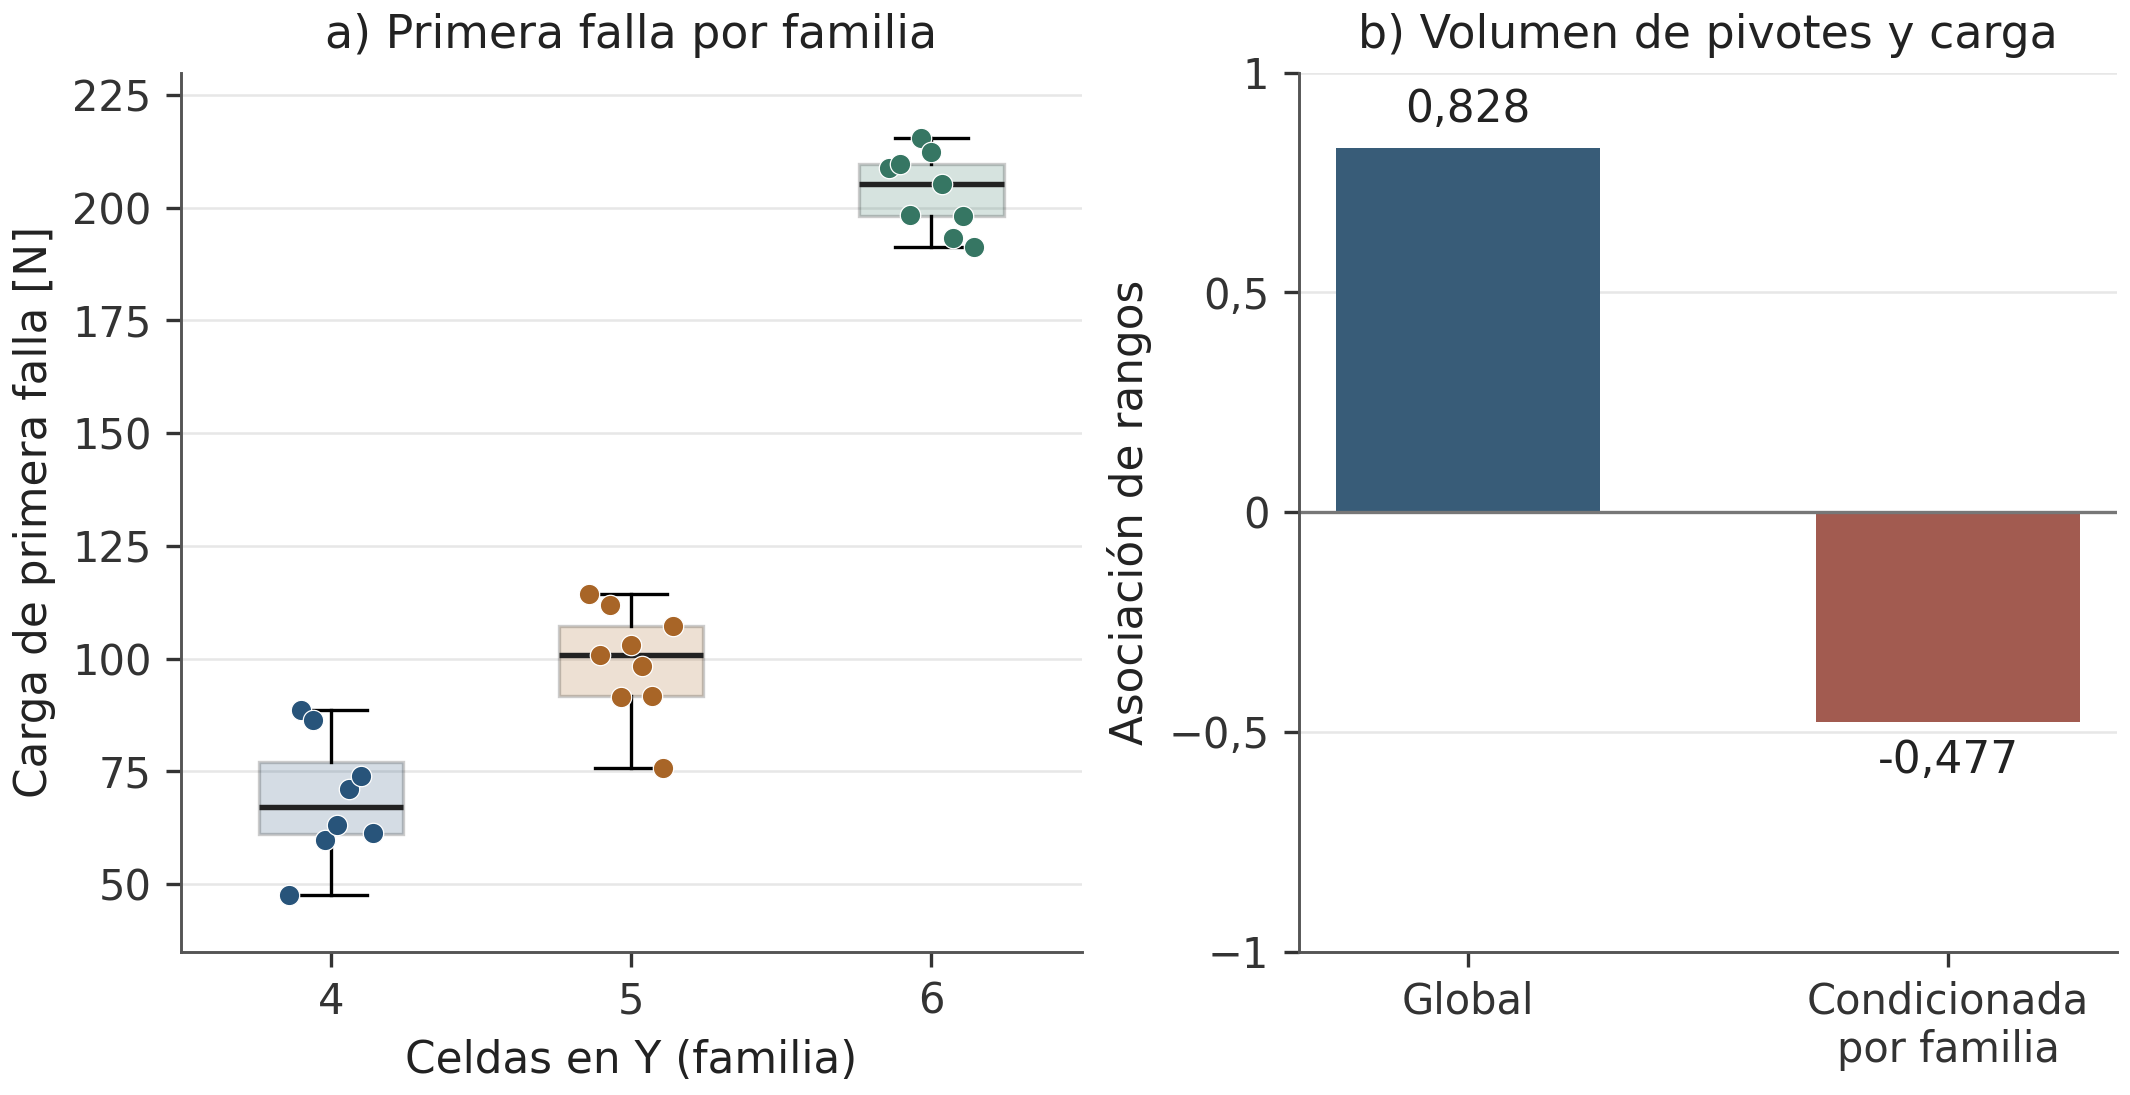
\includegraphics[width=\linewidth]{figures/04_eda.png}
\caption{Carga de primera falla por familia y asociaciones de volumen de pivotes con el objetivo. El coeficiente condicionado corresponde a rangos globales residualizados por familia; no es un promedio de correlaciones. Fuentes: tabla analítica y asociaciones del EDA.}
\label{fig:eda}
\end{figure}

\subsection{Síntesis EDA--Feature Engineering}
La Tabla~\ref{tab:eda-fe} conecta hallazgos e intervenciones. La asociación descriptiva propone hipótesis; la evaluación contrasta su utilidad. Como el EDA utiliza todos los objetivos, ajustar correctamente el pipeline no elimina el sesgo previo de selección \cite{cawley2010}.

\begin{table}[htbp]
\centering\small\setstretch{1.0}
\caption{Vinculación entre evidencia exploratoria y decisiones de ingeniería de características.}
\label{tab:eda-fe}
\begin{tabularx}{\linewidth}{@{}YYYYY@{}}
\toprule
Hallazgo EDA & Evidencia & Interpretación & Necesidad & Acción FE \\
\midrule
Forma de sección & Momentos con $\rho$ condicionado próximo a cero & Sin asociación condicionada fuerte; hipótesis geométrica & Evaluar términos no lineales dirigidos & Añadir ambos momentos en B \\
\addlinespace
Proporción de componentes & Log-razón: $\rho$ global 0,8280; condicionado $-0,4773$ & Asociación depende de familia & Contrastar representación relativa & Añadir $\ln(V_p/V_f)$ en C \\
\addlinespace
Dependencias de diseño & $V_f+V_p$ constante; longitud y pivotes asociados a familia & Descriptores dependientes & Probar parsimonia sin imponerla & Retirar un bloque de tres columnas en D \\
\addlinespace
Escalas y constante & mm, mm$^3$, conteos; radio 0,5~mm & Penalización sensible a unidades & Ajuste comparable y sin fuga & Filtrar constantes y escalar dentro de cada entrenamiento \\
\addlinespace
Dependencia y momento de medición & Factores repetidos; respuestas posteriores & Riesgo de evaluación optimista & Separar grupos y limitar entradas & Agrupar configuraciones; excluir respuestas e identificador \\
\bottomrule
\end{tabularx}
\par\smallskip\small Fuente: tablas de asociaciones, identidades, representaciones y matriz EDA--FE del repositorio. Los coeficientes son descriptivos; no expresan causalidad.
\end{table}

\section{Feature Engineering guiado por EDA}
\label{sec:fe}

\subsection{Justificación}
Ridge con ancho y altura separados combina $\beta_b b+\beta_h h$; no genera automáticamente $bh^3$ o $hb^3$. Añadir estos términos amplía las relaciones que puede representar: el estimador sigue siendo lineal en sus coeficientes, pero no en las medidas originales. Las nuevas columnas son funciones de geometría existente, no información experimental adicional. Su selección geométrica evita una expansión polinómica indiscriminada.

La penalización depende de la representación y la escala \cite{hoerl1970}: conjuntos algebraicamente relacionados pueden dar predicciones distintas. Retirar descriptores dependientes prueba si una representación menor conserva el desempeño; no garantiza mejorarlo.

\subsection{Características originales}
A parte de las entradas de la Tabla~\ref{tab:entradas}; el filtro entrenado elimina el radio y deja nueve predictores. La matriz original centrada tiene rango siete: los coeficientes no admiten una interpretación individual inequívoca, aunque Ridge permita ajustar el sistema. El ancho de fibra se conserva y alimenta los momentos; el identificador queda excluido.

\subsection{Características derivadas}
El primer bloque incorpora los segundos momentos de área de una sección rectangular ideal respecto de sus ejes centroidales:
\begin{equation}
I_{bh^3}=\frac{bh^3}{12},\qquad I_{hb^3}=\frac{hb^3}{12},
\label{eq:momentos}
\end{equation}
con $b,h$ en mm e $I$ en mm$^4$. Representan dos orientaciones de la sección; la literatura pantográfica fundamenta considerar geometría relacionada con flexión \cite{turco2017,turco2019}. No son rigidez $EI$ medida ni criterios de fractura, y no identifican el eje dominante de cada rotura. Se evalúan juntos: B--A estima el aporte del bloque, no la importancia individual.

Como control del cálculo, el caso 1 tiene $b=2{,}4$~mm y $h=1$~mm: las fórmulas producen 0,2 y 1,152~mm$^4$. La coincidencia con el pipeline verifica implementación, no validez mecánica ni mejora predictiva. Los momentos pueden ser redundantes con otras medidas y amplifican discrepancias del ancho o altura; su beneficio debe juzgarse con predicciones reservadas.

El segundo bloque añade
\begin{equation}
L_{p/f}=\ln\!\left(\frac{V_p}{V_f}\right)=\ln(V_p)-\ln(V_f),\qquad V_p,V_f>0.
\label{eq:logratio}
\end{equation}
La razón es adimensional y expresa proporción de volúmenes declarados. Su implementación usa diferencia de logaritmos, equivalente en el dominio positivo. No estima reparto de fuerzas ni asegura normalidad. Dada la complementariedad de volúmenes, no aporta una medición independiente: propone otra función no lineal de cantidades existentes. La inversión entre asociación global y condicionada motiva evaluarla sin anticipar una mejora.

La intervención final elimina longitud total de fibras, número de pivotes y volumen de fibras como columnas directas. Se conserva el conteo de celdas como descriptor de arquitectura y el volumen de fibras continúa siendo necesario para calcular $L_{p/f}$. Por tanto, D reduce entradas al regresor, pero no elimina la necesidad de disponer de ese volumen en el contrato de datos. El contraste evalúa conjuntamente simplificación y cambio de parametrización penalizada; no demuestra que cada columna retirada sea prescindible.

\subsection{Transformaciones estadísticas}
El pipeline aplica contrato geométrico, imputación, construcción de representación, filtro de varianza nula, estandarización y regresión \cite{pedregosa2011}. Las fórmulas y la lista de columnas de D son determinísticas. Las medianas de imputación y el filtro se calculan en entrenamiento; la imputación es una contingencia sin valores rellenados en la geometría actual. El objetivo nunca se imputa. El escalamiento utiliza
\begin{equation}
z_{ij}=\frac{x_{ij}-\mu_{j,\mathrm{train}}}{\sigma_{j,\mathrm{train}}},
\label{eq:escalamiento}
\end{equation}
con desviación poblacional del entrenamiento. Los casos reservados reutilizan esos parámetros. No se aplicaron codificación one-hot, transformación del objetivo, remuestreo sintético, selección supervisada adicional ni recorte de extremos. Los conteos conservan su valor numérico.

\subsection{Control de leakage}
El contrato admite exclusivamente las diez columnas geométricas, rechaza respuestas e identificadores y verifica positividad, finitud y conteos enteros. Cada partición crea un pipeline independiente; sus medianas, variables retenidas, medias, escalas e identificadores quedan registrados. La auditoría contrasta esas estadísticas con el entrenamiento efectivo y verifica que no se compartan casos ni grupos entre ajuste y evaluación. Las características derivadas no consultan el objetivo ni variables posteriores al ensayo.

Se controla la fuga de procesamiento, pero persiste el sesgo de formular hipótesis con todo el conjunto. La separación nominal tampoco certifica independencia física cuando faltan metadatos de lote o réplica.

\subsection{Feature sets experimentales}
Las variantes son acumulativas (Tabla~\ref{tab:featuresets}): B se contrasta con A, C con B y D con C. Cada paso modifica un bloque documentado, manteniendo el modelo, sus parámetros y las observaciones. No es un diseño factorial ni una ablación individual de todas las características.

\begin{table}[htbp]
\centering\small\setstretch{1.0}
\caption{Representaciones efectivamente evaluadas con Ridge. Los conteos corresponden a columnas tras retirar el radio constante.}
\label{tab:featuresets}
\begin{tabularx}{\linewidth}{@{}lYYYYY@{}}
\toprule
Set & Originales & Añadidas & Excluidas & Intervención & Justificación \\
\midrule
A (9) & Geometría original & Ninguna & Radio constante & Referencia & Error con dimensiones declaradas \\
\addlinespace
B (11) & Igual que A & Dos momentos & Radio constante & B--A: un bloque & Expansión no lineal de sección \\
\addlinespace
C (12) & Igual que A & Momentos y $L_{p/f}$ & Radio constante & C--B: una razón & Proporción entre componentes \\
\addlinespace
D (9) & A menos tres columnas & Igual que C & Radio, longitud, número de pivotes y $V_f$ directo & D--C: reducción de bloque & Parsimonia y parametrización \\
\bottomrule
\end{tabularx}
\par\smallskip\small Fuente: configuración y auditoría de transformaciones. La exclusión del radio pertenece al procesamiento común; $V_f$ sigue siendo insumo de la razón en D.
\end{table}

La decisión de conservar una característica se apoya en los errores reservados: interpretación física y dependencia algebraica justifican las pruebas, no anticipan su resultado.
